\documentclass[11pt]{article}
\usepackage[utf8]{inputenc}

%%% PAGE DIMENSIONS
\usepackage{geometry}
\geometry{a4paper}

\usepackage{graphicx}

%%% PACKAGES
\usepackage{booktabs}
\usepackage{paralist}
\usepackage{verbatim}
\usepackage{subfig}
\usepackage{chngcntr}
\usepackage{tikz}
\usepackage[colorlinks = true,
            linkcolor = black,
            urlcolor  = blue,
            citecolor = blue,
            anchorcolor = blue]{hyperref}
\usepackage[spanish]{cleveref}
\usepackage{placeins}
\usepackage{float}
\usepackage{listings}

%%% HEADERS & FOOTERS
\usepackage{fancyhdr}
\pagestyle{fancy}
\renewcommand{\headrulewidth}{0pt}
\lhead{}\chead{}\rhead{}
\lfoot{}\cfoot{\thepage}\rfoot{}

%%% SECTION TITLE APPEARANCE
\usepackage{sectsty}
\allsectionsfont{\sffamily\mdseries\upshape}

%%% ToC (table of contents) APPEARANCE
\usepackage[nottoc,notlof,notlot]{tocbibind} % Put the bibliography in the ToC
\usepackage[titles,subfigure]{tocloft} % Alter the style of the Table of Contents
\renewcommand{\cftsecfont}{\rmfamily\mdseries\upshape}
\renewcommand{\cftsecpagefont}{\rmfamily\mdseries\upshape} % No bold!


\graphicspath{ {images/} }

\counterwithin*{figure}{section}
\counterwithin*{figure}{subsection}
\counterwithin*{figure}{subsubsection}

\counterwithin*{table}{section}
\counterwithin*{table}{subsection}
\counterwithin*{table}{subsubsection}

\addtolength{\cftfignumwidth}{2em}

\renewcommand{\thefigure}{
  \ifnum\value{subsection}=0
    \thesection.\arabic{figure}
  \else
    \ifnum\value{subsubsection}=0
      \thesubsection.\arabic{figure}
    \else
      \thesubsubsection.\arabic{figure}
    \fi
  \fi
}

\renewcommand{\thetable}{
  \ifnum\value{subsection}=0
    \thesection.\arabic{table}
  \else
    \ifnum\value{subsubsection}=0
      \thesubsection.\arabic{table}
    \else
      \thesubsubsection.\arabic{table}
    \fi
  \fi
}

%%% END Article customizations

%%% The "real" document content comes below...

\title{\Large Seguridad en Redes\\Practica 3.4}
\author{David Antuña Rodríguez\\Javier Carrión García}
\date{}

\begin{document}
  \raggedright

  \maketitle
  \newpage

  \section{Sniffer y packet logger}
    \par
    El modo sniffer de snort tiene las siguientes opciones.
    \begin{itemize}
      \item -v\\
        Es la opción que permite iniciar snort en modo sniffer, imprimirá las
        cabeceras TCP/IP de los paquetes.
      \item -d\\
        Con esta opción snort también mostrara los datos no solo las cabeceras.
      \item -e\\
        Añadira a la información mostrada las cabeceras de la capa
        \textbf{data link}, la segunda de las siete que componen el modelo OSI.
    \end{itemize}

    \bigskip
    \par
    Si en lugar de sniffer queremos iniciar snort en modo packet logger tenemos
    que especificar el directorio en el que debe almacenar los paquetes, de este
    modo snort sabrá que debe iniciarse en modo packet logger.

    \begin{lstlisting}
      sudo snort -dev -l ./log
    \end{lstlisting}

  \section{NIDS basado en reglas}
    \begin{figure}[H]
      \centering
      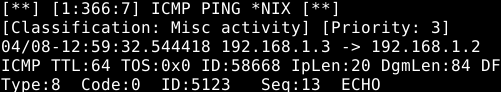
\includegraphics[width = \textwidth]{nbra}
    \end{figure}
    \par
    La regla con SID 366 estaba en el fichero
    \textit{/etc/snort/rules/icmp-info.rules}.
    \begin{lstlisting}
    alert icmp $EXTERNAL_NET any -> $HOME_NET any (msg:"ICMP PING *NIX";
    itype:8; content:"|10 11 12 13 14 15 16 17 18 19 1A 1B 1C 1D 1E 1F|";
    depth:32; classtype:misc-activity; sid:366; rev:7;)
    \end{lstlisting}

    \begin{figure}[H]
      \centering
      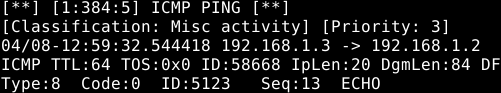
\includegraphics[width = \textwidth]{nbra1}
    \end{figure}
    \par
    La regla con SID 384 estaba en el fichero
    \textit{/etc/snort/rules/icmp-info.rules}.
    \begin{lstlisting}
    alert icmp $EXTERNAL_NET any -> $HOME_NET any (msg:"ICMP PING";
    icode:0; itype:8; classtype:misc-activity; sid:384; rev:5;)
    \end{lstlisting}

    \begin{figure}[H]
      \centering
      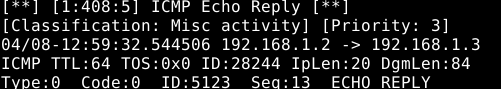
\includegraphics[width = \textwidth]{nbra2}
    \end{figure}
    \par
    La regla con SID 408 estaba en el fichero
    \textit{/etc/snort/rules/icmp-info.rules}.
    \begin{lstlisting}
    alert icmp $EXTERNAL_NET any -> $HOME_NET any (msg:"ICMP Echo Reply";
    icode:0; itype:0; classtype:misc-activity; sid:408; rev:5;)
    \end{lstlisting}

    \bigskip
    \par
    Para localizar las reglas hemos empleado el comando grep, tan solo es
    necesario decirle entre las comillas la cadena buscada en este caso el sid
    de la regla, en lugar de XXX se pone el SID a buscar. Al utilizar la opción
    "-r" realiza una busqueda en todos los ficheros del directorio.
    \begin{lstlisting}
    sudo grep -r "sid:XXX" /etc/snort/rules
    \end{lstlisting}

  \section{Definición de nuevas reglas}
    \begin{figure}[H]
      \centering
      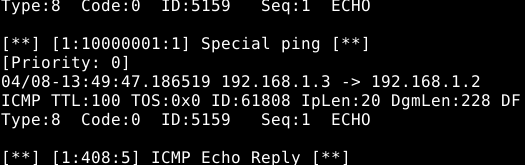
\includegraphics[width = \textwidth]{nra}
      \caption{Alerta generada por la nueva regla.}
    \end{figure}

    Para activarla hemos enviado un ping de atacante a victima pero lo hemos
    modificado para que tuviese el tiempo de vida y tamaño buscados.

    \begin{lstlisting}
      ping -t 100 -s 200 -c 1 192.168.1.2
    \end{lstlisting}

  \section{Preprocesadores}
    \begin{figure}[H]
      \centering
      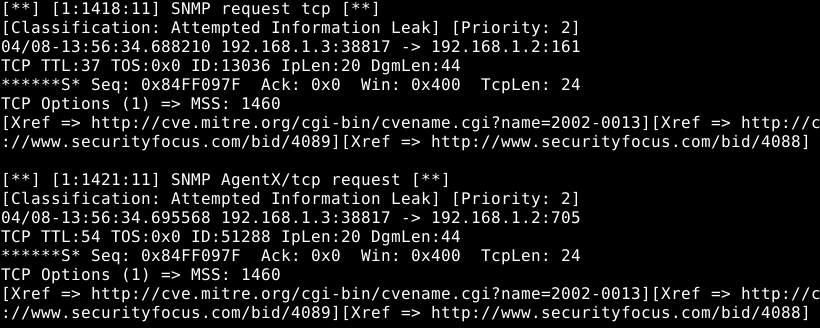
\includegraphics[width = \textwidth]{sfpa}
      \caption{Alerta con sfportscan activado.}
    \end{figure}

    Para activar el preprocesador arpspoof hemos incluido las siguientes lineas
    en el fichero \textit{/etc/snort/snort.conf}.
    \begin{lstlisting}
    preprocessor arpspoof
    preprocessor arpspoof_detect_host: 192.168.1.1 08:00:27:66:bf:ba
    preprocessor arpspoof_detect_host: 192.168.1.2 08:00:27:1f:21:c9
    preprocessor arpspoof_detect_host: 192.168.1.3 08:00:27:62:95:fc
    \end{lstlisting}

    \begin{figure}[H]
      \centering
      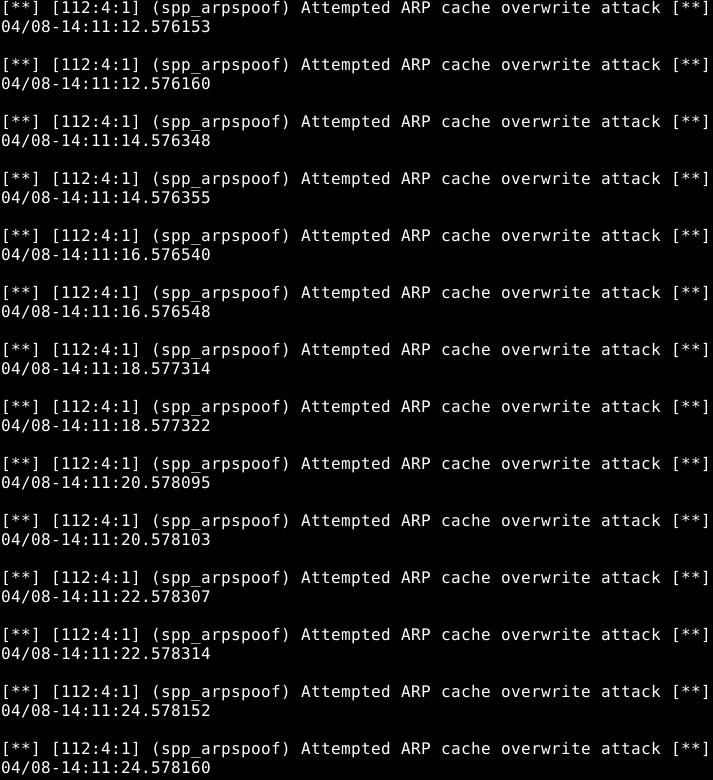
\includegraphics[width = \textwidth]{arpa}
      \caption{Alerta con arpspoof activado.}
    \end{figure}
\end{document}
